\section{Result}
\label{sec:result}
The following results are depending also on the hardware of the machine used.
The following tests were run on a  Intel(R) Core(TM) i7-3610QM CPU @ 2.30GHz.
In order to show the differences between the two implementations I selected some files
that you can find in the \verb|Sample| directory.
I wrote a script \verb|benchmark.sh| that runs
each instance of the problem ten times and then it computes the average
user time\footnote{In general the CPLEX API cpu time is much bigger(~7 time) than the genetic algorithm time
because CPLEX is multithreaded, the implementation of the second algorithm use only one thread}.
In order to test this problem, I used the 
following instances
\begin{itemize}
	\item TSP12, the tsp instance with 12 elements given during the class;
	\item TSP60, the tsp instance with 60 elements given during the class;
	\item REALWORLD, the real-world tsp instance, with data extrapolated from a real
	\verb|.gbr| file mentioned above;
	\item CIRCLE3-50 Circle instances 3 to 50
	\item RANDOM3-50 50 random but fixed instances, used in order to show the general-purpose efficiency of the genetic algorithms;
\end{itemize}
During the rest of the paper this names will be used.

\subsection{Result - First Assignment}
In this part of the port the focus is put on the performance of the exact solution.
The result of the exact solution can be found in the corresponding images

\paragraph{CIRCLE3-50}
The result of this benchmark are quite surprisingly because
the time does not grow proportionally with the increase of $N$.
Note especially the entries 37,41,47 requires a very small amount of time. Instead
there are also entries that do not work good, such as 49 and 64\footnote{It was excluded because even on the
lab computer it required more than 42 minutes (I did not a get a result)}.

\paragraph{RANDOM3-50}
The result of this benchmark shows that when $N$ increases the time required
grows accordingly, but there are some exceptions.

\paragraph{TSP12, TSP60, RealWorld}
The TSP60 and the RealWorld example consists of circa the same number of points and
therefore required a time in the same order of magnitude.


\begin{figure}
	\centering
	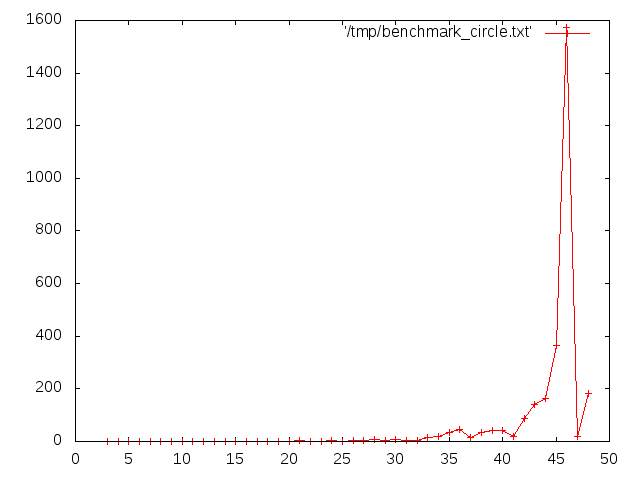
\includegraphics[scale=0.4]{img/benchmark_circle.png}
	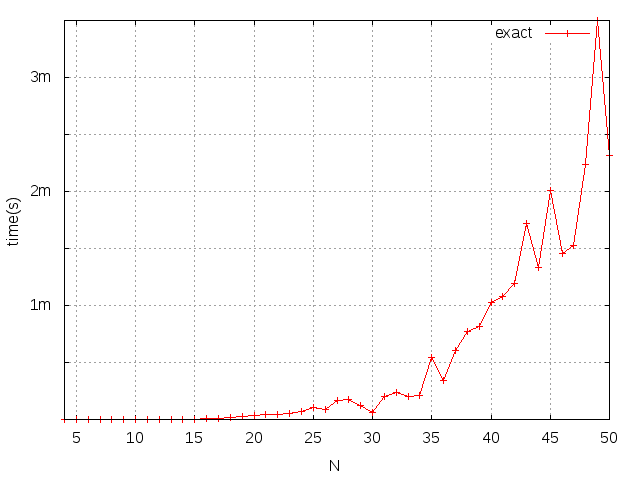
\includegraphics[scale=0.4]{img/firstAssignment/RANDOMTSPINSTANCE.png}
	\caption{The time result of the benchmark CIRCLE3-50, RANDOM3-50}
\end{figure}
In general from the above graphs I concluded:
\begin{itemize}
	\item That with a small $N$ (from 3 to 30) the program performs very well
	\item The program works better with solutions that are generated randomly, i.e. with points distributed 
	across the whole board. Instead it requires (generally) more time when the points are grouped
	in the corners of the board. More importantly when this is the case the performance of the CPLEX
	API becomes very unstable (you can consider $N = 46$ and $N=47$ as an example).
\end{itemize}
\newpage


\section{Result - Second Assignment}



\section{Result-Second Assignment}
The time required by the second assignment is not so  trustworthy 
as the first one, because it depends strongly about the random
generated population. Therefore this section is divided in two
parts: the first treats the time required by the algorithm and
the second one compare the objective value provided by the exact
solution with the one found with the genetic algorithm. During the
10 run I take the best the worst and the average one.
\subsection{Performance}
As already mentioned this approach relies on the random choices made during the execution but 
also on the population size, the number of elements generated.
In general it is much faster as you can see in the graphs \ref{fig:comparison}
and therefore it does not make sense to compare the first and the second
algorithm on the basis of efficiency.

\begin{figure}
	\label{fig:comparison}
	\centering
	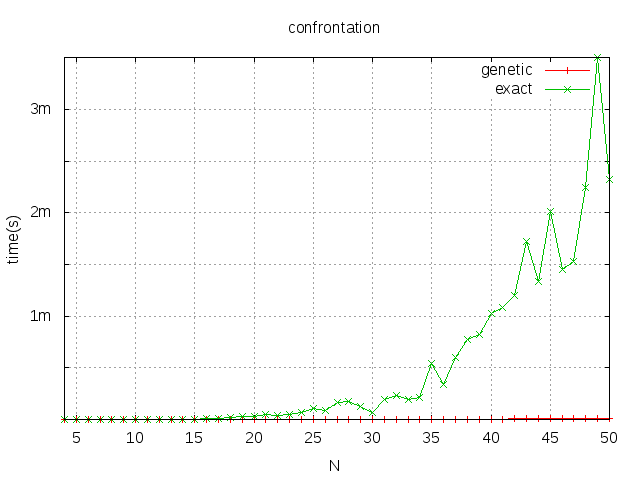
\includegraphics[scale=0.5]{img/confronto_random_exact_genetic.png}
\end{figure}

\begin{figure}
	\centering
	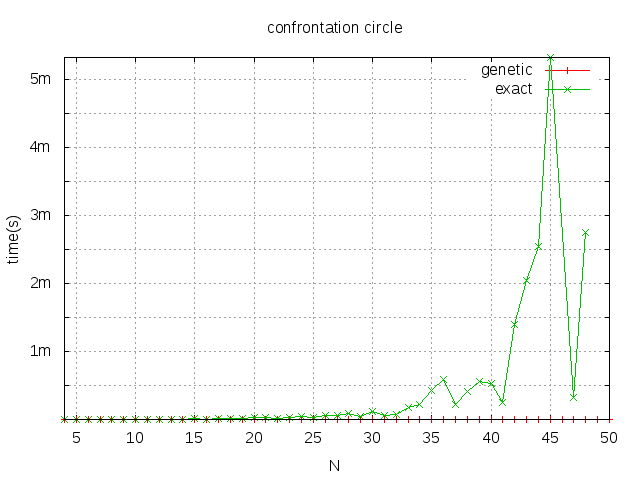
\includegraphics[scale=0.5]{img/confronto_circle_exact_genetic.png}
	\caption{N.B. the input 46 was removed because it required more than 23 minutes.}
\end{figure}

\subsection{Quality of the result}
Inside this section the result provided by the genetic algorithm are compared with
those generated by the exact solution.
Each graph contains the average result.

\section{Comparison between Solution I and Solution II}
It does not make to much sense to compare the metaheuristic and the
exact approach on a time based, because the genetic algorithm is faster.

